\label{subsec:partycjonowanie}
Partycjonowanie to proces zmiany układu partycji na dysku twardym. Jest to najważniejszy etap instalacji systemu, gdyż od niego w dużej mierze zależy to, jak system będzie działał. Pamiętaj, że na tym etapie pracujesz na danych zapisanych na dysku twardym. Chwila nieuwagi może spowodować ich utratę.
\subsubsection{Ile miejsca przeznaczyć na Ubuntu}
\label{ile_miejsca}
Wirtualny dysk twardy użyty w tym przewodniku ma tylko 26,8 gigabajta pojemności. Twój dysk twardy zapewne będzie miał kilkaset gigabajtów (jeżeli nie kilka terabajtów) pojemności. Dlatego też liczby, jakimi się tu posługujemy, będą miały niewielkie przełożenie na sytuację na twoim komputerze. W tym miejscu powinieneś się jednak zastanowić, ile miejsca chcesz przeznaczyć na Ubuntu.
Ogólnie rzecz ujmując, sprawa wygląda następująco:
\begin{itemize}
\item \textcolor{ubuntu_orange}{Partycja główna, root, /} --- 6,2 gigabajta to absolutne minimum. 10 gigabajtów da pewną elastyczność i pozwoli zainstalować więcej programów. Nie ma potrzeby przesadzać w drugą stronę i tworzyć zbyt dużą partycję główną, gdyż wolna przestrzeń będzie niewykorzystana. 15 -- 20 gigabajtów w~zupełności wystarczy.
\item \textcolor{ubuntu_orange}{Partycja wymiany, swap} --- na tej partycji zapisywane są dane, które nie mieszczą się w pamięci operacyjnej. Tutaj też przechowywany jest obraz RAM-u, kiedy poddajesz komputer hibernacji. Jeżeli korzystasz z hibernacji, to wielkość partycji swap powinna być co najmniej taka, jak ilość pamięci operacyjnej twojego komputera. Jeżeli nie planujesz korzystać z hibernacji, to możesz nie tworzyć partycji wymiany. Jednak zaleca się jej stworzenie, jeżeli masz mniej niż 2 gigabajty RAM-u. W~takim wypadku, nawet jeżeli nie korzystasz z hibernacji, to dobrze jest stworzyć niewielką (300 --- 400 megabajtów) partycję swap.
\item \textcolor{ubuntu_orange}{Partycja domowa, /home} --- W katalogu /home przechowywane są prywatne pliki użytkownika: zawartość pulpitu, dokumenty, filmy, muzyka i ustawienia programów. Katalog domowy może znajdować się na głównej partycji (/, root) lub można go wydzielić. Dobrą praktyką jest wydzielenie takiej partycji, gdyż w razie reinstalacji systemu nie trzeba będzie jej kasować. Nadpisana zostanie tylko partycja główna, zaś wszystkie prywatne dane pozostaną niezmienione. Wielkość tej partycji zależy tylko i wyłącznie od tego, jak wiele miejsca chcesz na nią przeznaczyć i jak wiele rzeczy zamierzasz na niej trzymać. 
\end{itemize}
\clearpage
\subsubsection{Czysty dysk --- wykorzystanie całego dostępnego miejsca}
\begin{center}
	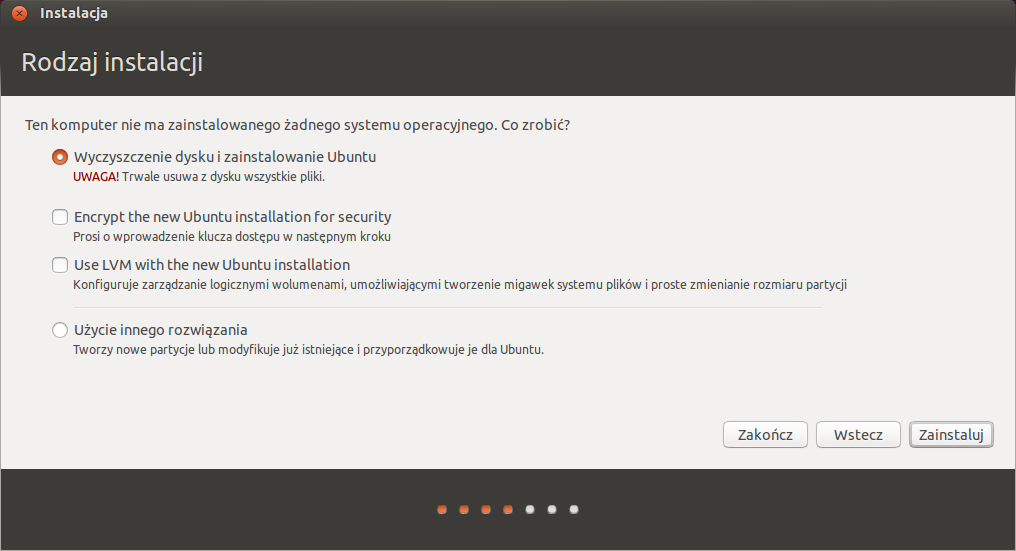
\includegraphics[width=\linewidth]{images/instalator_partycjonowanie_proste.png}
\end{center}

Jeżeli na dysku twardym nie ma żadnego innego systemu operacyjnego, instalator Ubuntu zaproponuje wykorzystanie całej dostępnej przestrzeni. Instalator sam dobierze odpowiedni rozmiar partycji systemowej, partycji wymiany oraz partycji użytkownika.
\begin{flushright}
Kliknij przycisk \textcolor{ubuntu_orange}{Zainstaluj}, aby przejść dalej.\\
Zostaniesz poproszony o potwierdzenie.\\
Upewnij się, że wszystko jest w porządku i kliknij \textcolor{ubuntu_orange}{Naprzód}.\\
W tym momencie wybrane zmiany zostaną zapisane na dysku twardym.
\end{flushright}
\clearpage
\subsubsection{Instalacja obok zainstalowanego Ubuntu}
\begin{center}
	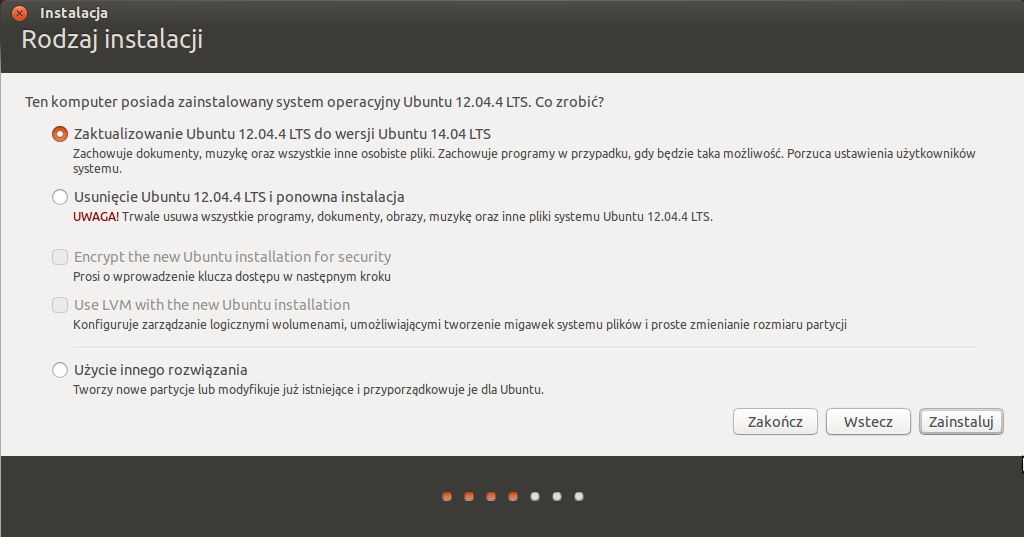
\includegraphics[width=\linewidth]{images/instalator_partycjonowanie_obok_ubuntu.png}
\end{center}

Jeżeli instalator wykryje obecność wcześniej zainstalowanej innej wersji Ubuntu, to zaproponuje kilka innych rozwiązań.
Pierwszym z nich jest aktualizacja zainstalowanego systemu do najnowszego wydania. Wszystkie dane w katalogu domowym użytkownika zostaną zachowane: muzyka, filmy, dokumenty, pliki na pulpicie, osobiste ustawienia programów, zakładki i historia przeglądarki, itp.

Skasowane zostaną zainstalowane w systemie programy oraz ustawienia systemowe. Instalator zaktualizuje istniejące na dysku oprogramowanie i ewentualnie pobierze aktualizacje z internetu (jeżeli wybrałeś wcześniej tę opcję).
Drugą z możliwości jest usunięcie zainstalowanego Ubuntu i ponowna instalacja systemu. Wszystkie dane zostaną wymazane.
\begin{flushright}
Kliknij przycisk \textcolor{ubuntu_orange}{Zainstaluj}, aby przejść dalej.\\
Zostaniesz poproszony o potwierdzenie.\\
Upewnij się, że wszystko jest w porządku i kliknij \textcolor{ubuntu_orange}{Naprzód}.\\
W tym momencie wybrane zmiany zostaną zapisane na dysku twardym.
\end{flushright}
\clearpage
\subsubsection{Instalacja obok Windowsa}
\begin{center}
	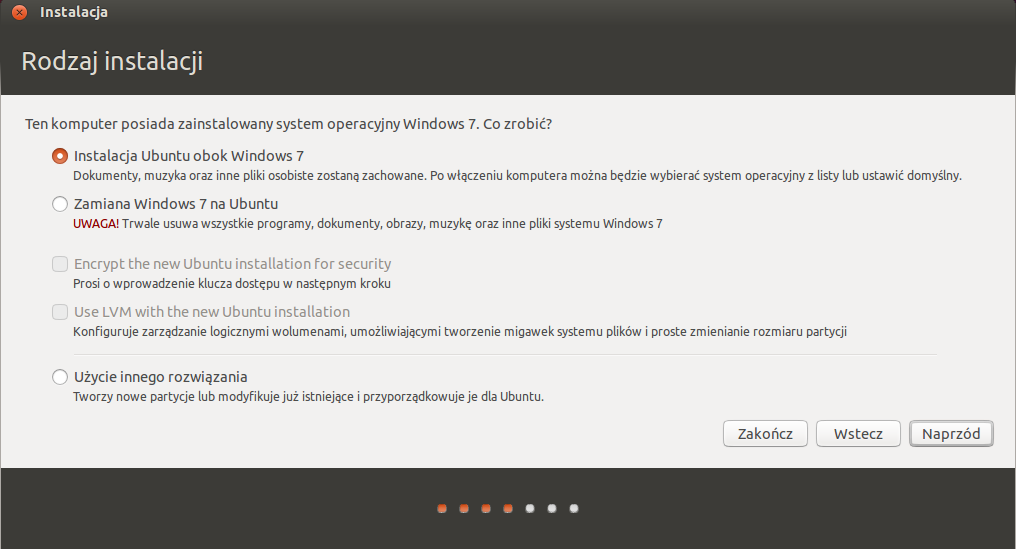
\includegraphics[width=\linewidth]{images/instalator_partycjonowanie_obok_wondows7.png}
\end{center}

Jeżeli instalator wykryje obecność wcześniej zainstalowanego systemu Windows, to zaproponuje inne rozwiązanie. ,,Zamiana Windows na Ubuntu'' wymaże całą zawartość partycji Windows (wraz ze wszystkimi danymi) i w to miejsce zainstaluje Ubuntu. Zostało to opisane dwie strony wcześniej.
\begin{flushright}
Kliknij przycisk \textcolor{ubuntu_orange}{Zainstaluj}, aby przejść dalej.
\end{flushright}

\begin{center}
\begin{tikzpicture}
	\node[anchor=south west,inner sep=0] (image) at (0,0) {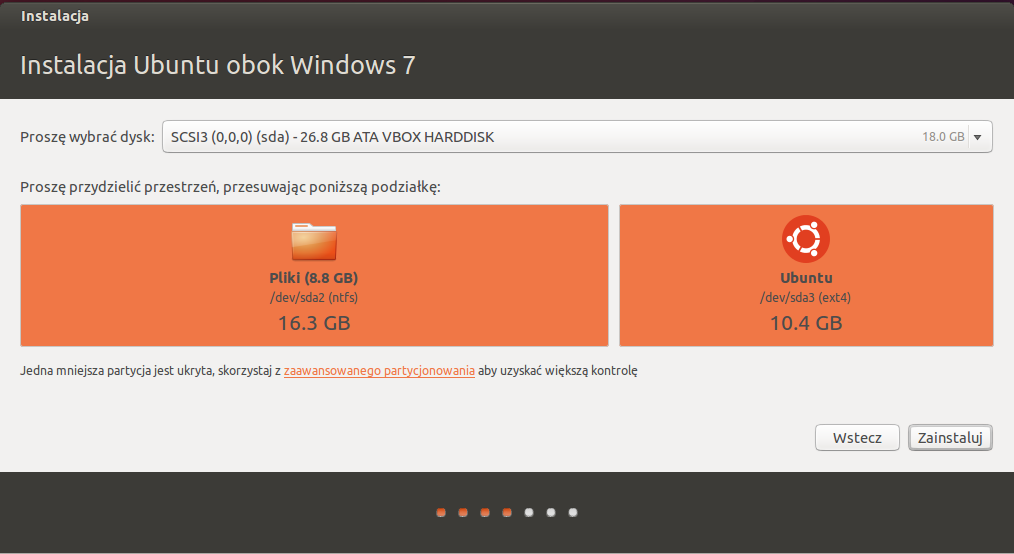
\includegraphics[width=\linewidth]{images/instalator_partycjonowanie_obok_wondows7_2.png}};
	\begin{scope}[x={(image.south east)},y={(image.north west)}]
		\draw[ubuntu_orange,line width=3pt,rounded corners] (0.16,0.72) rectangle (0.98,0.79);
		\draw[ubuntu_orange,line width=3pt,fill=white,fill opacity=0.75] (0.55,0.85) circle [radius=0.30cm]
			node[text=black]{\Large \textbf 1};
		\draw[ubuntu_orange,dashed,line width=3pt] (0.55,0.81) -- (0.55,0.79);	
	
		\draw[ubuntu_orange,line width=1.5pt,decorate,decoration={brace,amplitude=12pt,mirror}] (0.02,0.36) -- (0.6,0.36);
		\draw[ubuntu_orange,line width=3pt,fill=white,fill opacity=0.75] (0.31,0.24) circle [radius=0.30cm]
			node[text=black]{\Large \textbf 2};
		\draw[ubuntu_orange,line width=1.5pt,decorate,decoration={brace,amplitude=12pt,mirror}] (0.61,0.36) -- (0.98,0.36);
		\draw[ubuntu_orange,line width=3pt,fill=white,fill opacity=0.75] (0.795,0.24) circle [radius=0.30cm]
			node[text=black]{\Large \textbf 3};
    \end{scope}
\end{tikzpicture}
\end{center}

Drugą możliwością jest instalacja Ubuntu obok już zainstalowanego systemu Windows. Jeżeli wybierzesz tę opcję, to następny ekran pozwoli wybrać o ile instalator ma zmniejszyć partycję, na której zainstalowany jest system Windows. Menu \circled 1 pozwala wybrać dysk dwardy, na którym mają zostać dokonane operacje. Użyj myszy, aby przesunąć pomarańczową podziałkę w lewo (więcej miejsca dla Ubuntu) lub w prawo (więcej miejsca dla Windows). Oryginalna partycja systemu Windows jest oznaczona na tym obrazie jako ,,Pliki'' \circled 2. Partycja dla Ubuntu na powyższym obrazku to \circled 3. Pamiętaj, że Ubuntu potrzebuje minimum 6,2 gigabajta przestrzeni, ale tak mała partycja zostanie prawie w całości wypełniona przez system i na twoje pliki pozostanie niewiele miejsca.
\begin{flushright}
Kliknij przycisk \textcolor{ubuntu_orange}{Zainstaluj}, aby przejść dalej.\\
Zostaniesz poproszony o potwierdzenie.\\
Upewnij się, że wszystko jest w porządku i kliknij \textcolor{ubuntu_orange}{Naprzód}.\\
W tym momencie wybrane zmiany zostaną zapisane na dysku twardym.
\end{flushright}

\subsubsection{Szyfrowanie dysku twardego}
\begin{center}
	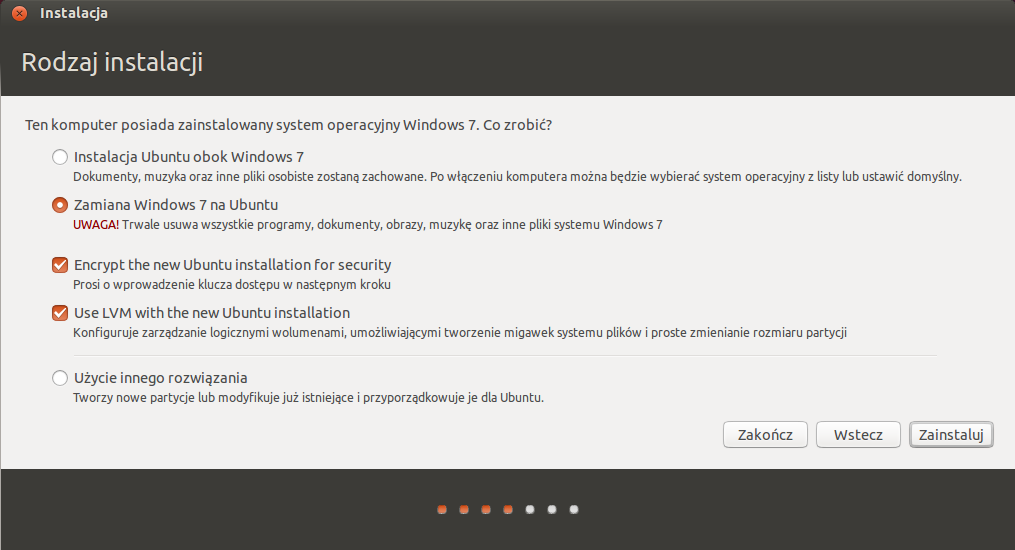
\includegraphics[width=\linewidth]{images/instalator_partycjonowanie_szyfrowanie1.png}
\end{center}

Przy wyborze jednego z automatycznych rozwiązań partycjonowania miałeś możliwość zastosowania szyfrowania dysku twardego. Jeśli wybierzesz tę opcję, zostanie wyświetlone okno jak na powyższym obrazku. Zaszyfrowanie dysku twardego sprawi, że nikt nie uzyska dostępu do twoich danych, ani nie zmodyfikuje zainstalowanego systemu. Wadą tego rozwiązania jest pewne zwiększenie obciążenia procesora i związane z tym zmniejszenie płynności działania komputera. Nowoczesne procesory zapewniają akcelerację sprzętową dla obliczeń kryptograficznych, w związku z czym utrata wydajności będzie się mieścić w granicach 5\% przy intensywnych operacjach dyskowych.
\begin{flushright}
Kliknij przycisk \textcolor{ubuntu_orange}{Zainstaluj}, aby przejść dalej.
\end{flushright}

\begin{center}
	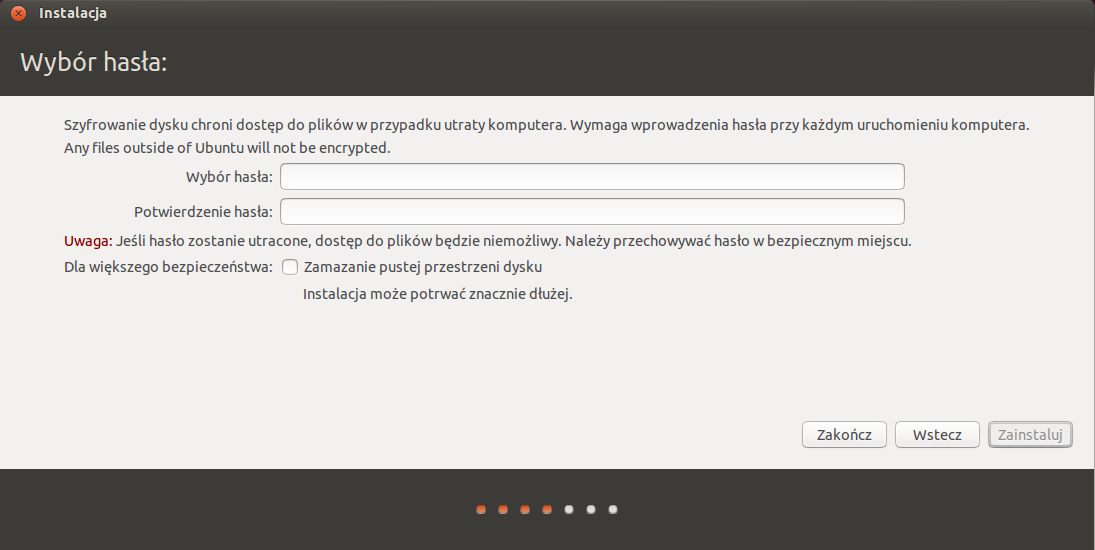
\includegraphics[width=\linewidth]{images/instalator_partycjonowanie_szyfrowanie2.png}
\end{center}

W tym miejscu podaj hasło --- klucz do dysku twardego. To nie jest to samo hasło, które ustawisz do swojego systemowego konta, a hasło umożliwiające dostęp do danych zapisanych na dysku twardym. Pamiętaj, że jeżeli zapomnisz wprowadzone tu hasło, nie będzie możliwości odzyskania zaszyfrowanych danych. Postaraj się też, aby hasło było trudne do odgadnięcia, ale łatwe do zapamiętania przez ciebie.

Opcja ,,Zamazanie pustej przestrzeni dysku'' powoduje, że niewykorzystywana, wolna przestrzeń dysku zostanie nadpisana losowymi danymi. Taka operacja znacznie utrudnia potencjalnym włamywaczom odczytanie twoich danych. Miej na uwadze, że zamazywanie pustej przestrzeni może trwać bardzo długo, w zależności od tego, ile miejsca przeznaczysz na Ubuntu.
\begin{flushright}
Kliknij przycisk \textcolor{ubuntu_orange}{Zainstaluj}, aby przejść dalej.\\
Zostaniesz poproszony o potwierdzenie.\\
Upewnij się, że wszystko jest w porządku i kliknij \textcolor{ubuntu_orange}{Naprzód}.
W tym momencie wybrane zmiany zostaną zapisane na dysku twardym.\\
\end{flushright}
\clearpage
\subsection{Zaawansowane partycjonowanie}
\begin{center}
	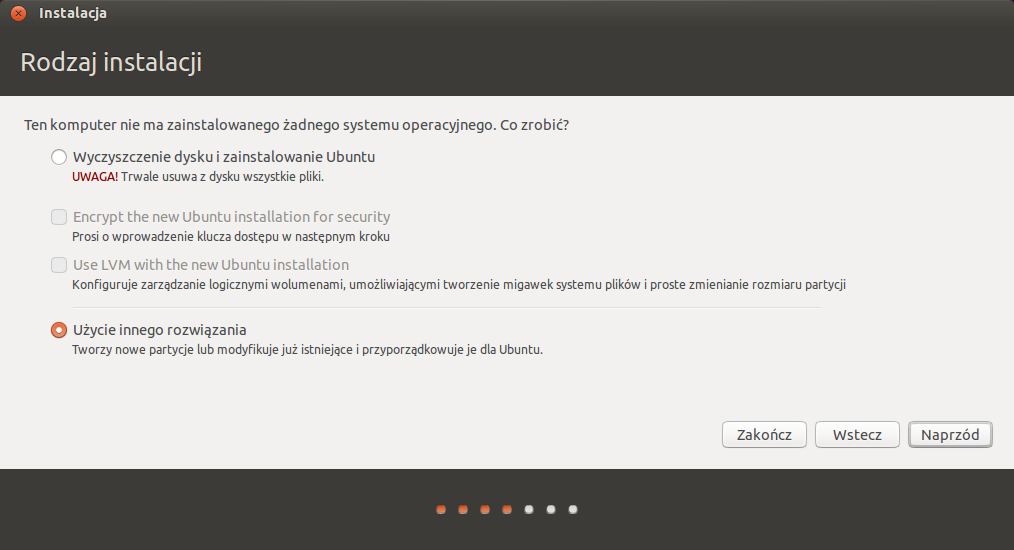
\includegraphics[width=\linewidth]{images/instalator_partycjonowanie_gparted1.png}
\end{center}

\textcolor{ubuntu_orange}{Użycie innego rozwiązania} uruchamia program GParted, który umożliwia nieograniczone modyfikowanie partycji na dysku twardym. Jest to opcja dla bardziej zaawansowanych użytkowników, którzy mają świadomość tego, jak działa partycjonowanie i jak powinien zostać podzielony ich dysk twardy. Jeżeli na swoim komputerze masz zainstalowany więcej niż jeden system operacyjny lub z jakiegoś innego powodu przedstawione wcześniej opcje nie spełniają twoich wymagań, to konieczne będzie zastosowanie zaawansowanego partycjonowania.

Do GParted warto zajrzeć z jeszcze jednego powodu. Podział partycji stosowany przez automatyczną instalację nie jest idealny. Ręczne ustawienie partycji da większą kontrolę i pozwoli znacznie lepiej dopasować układ partycji.
\begin{flushright}
Kliknij przycisk \textcolor{ubuntu_orange}{Naprzód}, aby przejść dalej.
\end{flushright}
\clearpage
\subsubsection{Główne okno programu GParted}
\begin{center}
\begin{tikzpicture}
	\node[anchor=south west,inner sep=0] (image) at (0,0) {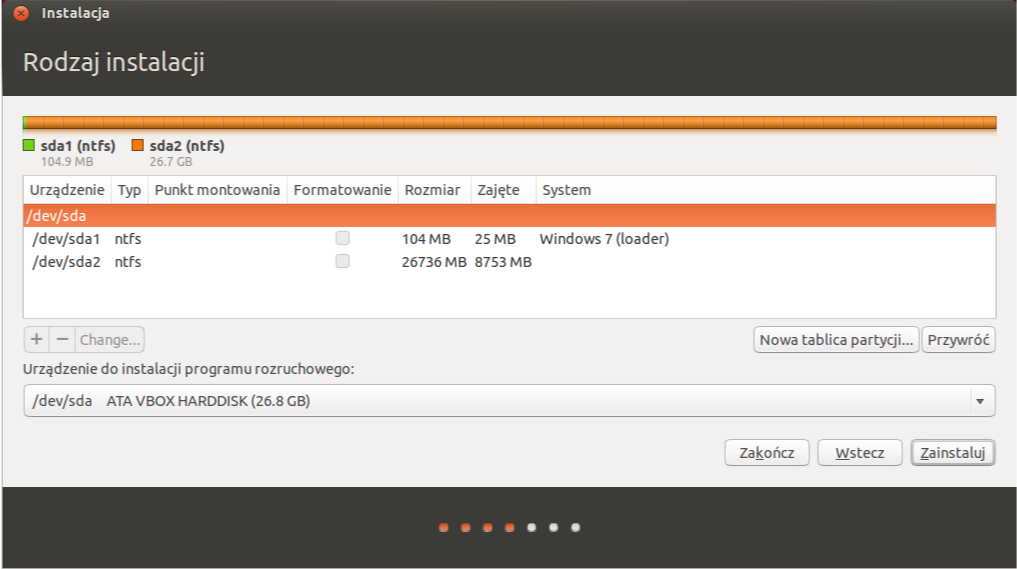
\includegraphics[width=\linewidth]{images/instalator_partycjonowanie_gparted2_czysty.png}};
	\begin{scope}[x={(image.south east)},y={(image.north west)}]
		\draw[ubuntu_orange,line width=3pt,rounded corners] (0.01,0.76) rectangle (0.99,0.81);
		\draw[ubuntu_orange,line width=3pt,fill=white,fill opacity=0.75] (0.45,0.90) circle [radius=0.30cm]
			node[text=black]{\Large \textbf 1};
		\draw[ubuntu_orange,dashed,line width=3pt] (0.45,0.87) -- (0.45,0.81);
		
		\draw[ubuntu_orange,line width=3pt,rounded corners] (0.01,0.45) rectangle (0.99,0.70);
		\draw[ubuntu_orange,line width=3pt,fill=white,fill opacity=0.75] (0.75,0.55) circle [radius=0.30cm]
			node[text=black]{\Large \textbf 2};
			
		\draw[ubuntu_orange,line width=3pt,rounded corners] (0.01,0.38) rectangle (0.15,0.43);
		\draw[ubuntu_orange,line width=3pt,fill=white,fill opacity=0.75] (0.35,0.35) circle [radius=0.30cm]
			node[text=black]{\Large \textbf 3};
		\draw[ubuntu_orange,dashed,line width=3pt] (0.33,0.35) -- (0.15,0.40);
    \end{scope}
\end{tikzpicture}
\end{center}

Na powyższym obrazku widzisz główne okno programu GParted. Wykryty został układ partycji na dysku twardym. Poziomy pasek \circled 1, rozciągający się na całą szerokość okna, jest graficzną reprezentacją układu partycji. Poniżej paska znajduje się legenda objaśniająca użyte kolory. Tabela \circled 2, znajdująca się w centralnej części okna, przedstawia szczegółowe informacje na temat partycji na dysku twardym. Zestaw przycisków \circled 3 służy do dodawania (\textcolor{ubuntu_orange}{+}), usuwania (\textcolor{ubuntu_orange}{-}) lub modyfikacji partycji(\textcolor{ubuntu_orange}{Change}). W tej chwili inne rzeczy nas nie interesują.

Powyższy układ dysków twardych oraz partycji jest tylko przykładem skonstruowanym na maszynie wirtualnej. Na twoim komputerze liczby będą inne.

Tabela umieszczona w centrum tego okna przedstawia informacje o poszczególnych partycjach obecnych na dysku twardym. Oto objaśnienie poszczególnych kolumn:
\begin{itemize}
\item \textcolor{ubuntu_orange}{Urządzenie} --- ścieżka do poszczególnych partycji na dysku twardym. Są to oznaczenia stosowane w systemach uniksowych (do których należy Linux, a więc i Ubuntu)), opisujące jak rozpoznawane są poszczególne partycje. W tym wypadku:
        \begin{itemize}
        \item \textcolor{ubuntu_orange}{/dev/} --- skrót od ,,Device'', urządzenie;
        \item \textcolor{ubuntu_orange}{sda} --- oznaczenie pierwszego dysku twardego;
                \begin{itemize}
                        \item \textcolor{ubuntu_orange}{sd} --- dysk na złączu SATA (sata disk);
                        \item \textcolor{ubuntu_orange}{a} --- pierwszy dysk; drugi dysk twardy miałby literę ,,b'', trzeci ,,c'', i tak dalej;
                \end{itemize}
        \item \textcolor{ubuntu_orange}{sda1} --- pierwsza partycja na pierwszym dysku twardym;
        \item \textcolor{ubuntu_orange}{sda2} --- druga partycja na pierwszym dysku twardym.
        \end{itemize}
\item \textcolor{ubuntu_orange}{Typ} --- rodzaj systemu plików. Sposób, w jaki partycja została sformatowana. System Windows korzysta z NTFS, Ubuntu może korzystać z różnych.
\item \textcolor{ubuntu_orange}{Punkt montowania} --- miejsce, w którym dana partycja zostanie ,,zamontowana'', katalog, w którym będzie widoczna zawartość tej partycji.
\item \textcolor{ubuntu_orange}{Formatowanie} --- zaznaczając to pole informujesz instalator, że dana partycja ma zostać sformatowana. Oznacza to utratę wszystkich danych na niej zapisanych.
\item \textcolor{ubuntu_orange}{Rozmiar} --- pojemność partycji w megabajtach.
\item \textcolor{ubuntu_orange}{Zajęte} --- ilość zajętego miejsca na partycji.
\item \textcolor{ubuntu_orange}{System} --- system operacyjny zainstalowany na danej partycji. Nie zawsze da się rozpoznać zainstalowany system. Nie każda partycja musi mieć zainstalowany system operacyjny. 
\end{itemize}

\subsubsection{Zaawansowane partycjonowanie --- instalacja obok systemu Windows}
\begin{center}
	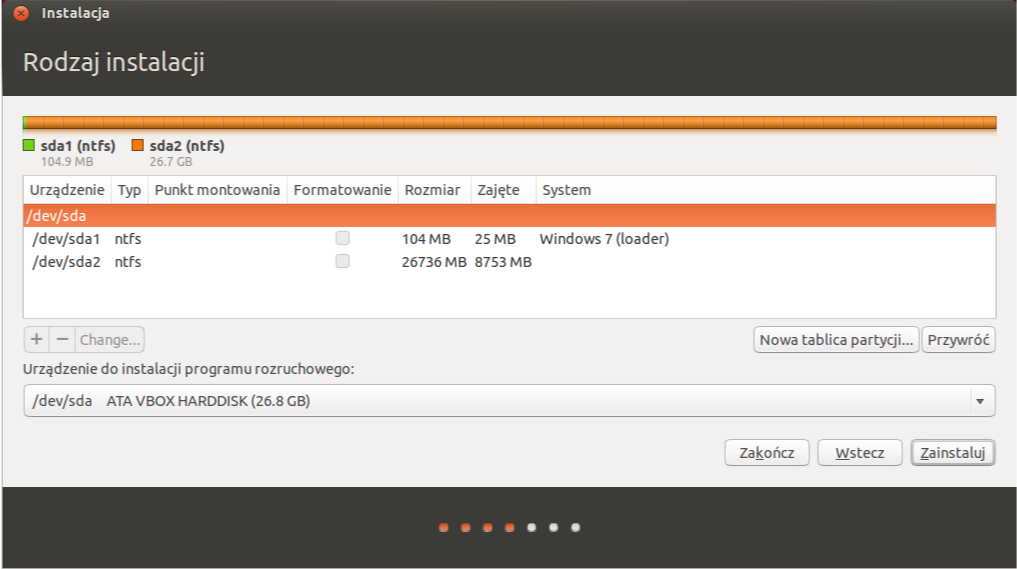
\includegraphics[width=\linewidth]{images/instalator_partycjonowanie_gparted2_czysty.png}
\end{center}

Na powyższym obrazku widać dwie partycje utworzone przez instalator systemu Windows 7. Partycja zielona o rozmiarze 104 megabajtów służy jako partycja programu rozruchowego systemu Windows. Duża, pomarańczowa partycja (26736 megabajtów) to główna partycja systemu Windows 7. Bardzo podobny układ partycji stosowany jest przez każdy z systemów z rodziny Windows.\\
Pierwszym krokiem jest wydzielenie miejsca dla systemu Ubuntu. Kliknij na partycji \textcolor{ubuntu_orange}{/dev/sda2}. Następnie kliknij przycisk \textcolor{ubuntu_orange}{Change}, znajdujący się pod tabelą. W otwartym oknie możesz zmniejszyć rozmiar wybranej partycji.

\begin{wrapfigure}{R}{0.5\textwidth}
	\vspace{-10pt}
	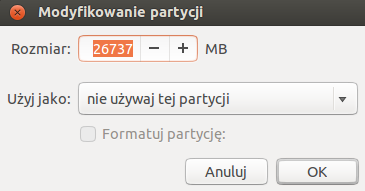
\includegraphics[width=\linewidth]{images/instalator_partycjonowanie_gparted_zmniejszenie_partycji_windows.png}
\end{wrapfigure}

W polu \textcolor{ubuntu_orange}{Rozmiar} podaj nowy rozmiar partycji. O tym ile miejsca potrzebujesz na Ubuntu przeczytasz w rozdziale \ref{ile_miejsca} ,,Ile miejsca przeznaczyć na Ubuntu''. W polu podajesz rozmiar partycji w megabajtach. Jeden gigabajt to 1024 megabajty.

Upewnij się, że wybrano opcję \textcolor{ubuntu_orange}{nie używaj tej partycji}. Teraz kliknij przycisk \textcolor{ubuntu_orange}{OK}, a następnie \textcolor{ubuntu_orange}{Naprzód}, aby dokonać zmiany na partycji. Wykonanie żądanej zmiany może trwać dłuższą chwilę.

\begin{center}
	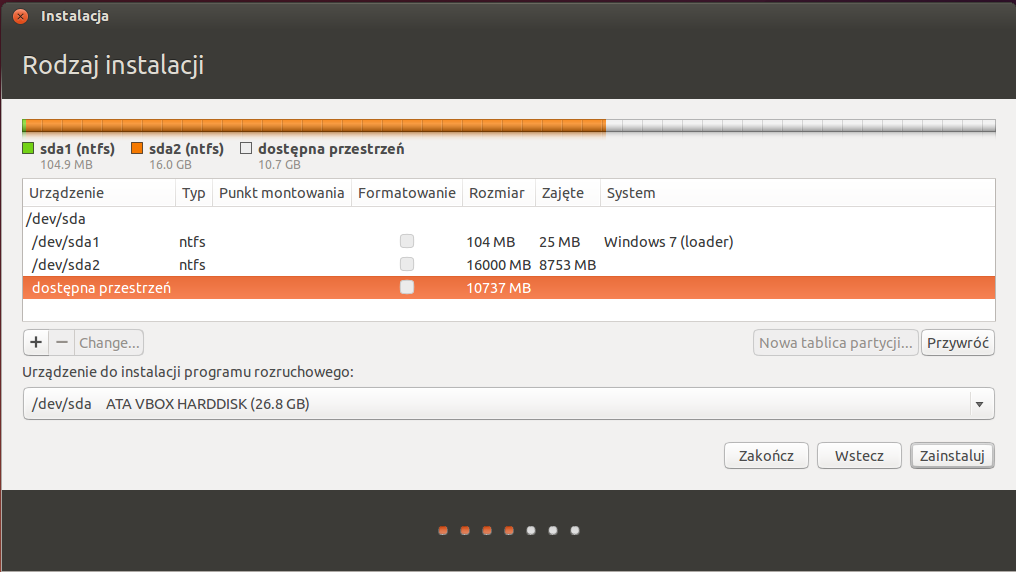
\includegraphics[width=\linewidth]{images/instalator_partycjonowanie_gparted3.png}
\end{center}

\begin{wrapfigure}[9]{R}{0.5\textwidth}
	\vspace{-10pt}
	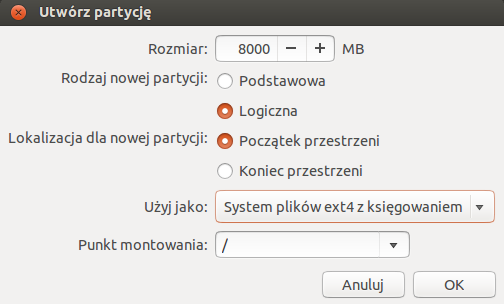
\includegraphics[width=\linewidth]{images/instalator_partycjonowanie_gparted_dodaj_root.png}
	\caption*{Ustawienia dla partycji głównej (/).}
\end{wrapfigure}

Na schemacie pojawiła się pusta, oznaczona kolorem szarym \textcolor{ubuntu_orange}{dostępna przestrzeń}. Zaznacz ją, a następnie kliknij przycisk (\textcolor{ubuntu_orange}{+}), aby stworzyć nową partycję.

Na początku musimy stworzyć partycję podstawową dla Ubuntu. O ilości miejsca potrzebnego na poszczególne partycje przeczytasz w sekcji \ref{ile_miejsca} ,,Ile miejsca przeznaczyć na Ubuntu''. Pozostałe opcje ustaw, jak na rysunku.
\begin{itemize}
\item \textcolor{ubuntu_orange}{Rozmiar} --- rozmiar partycji w megabajtach.
\item \textcolor{ubuntu_orange}{Rodzaj nowej partycji} --- system Windows korzysta z tablicy partycji MS-DOS, więc jesteśmy ograniczeni do 4 partycji podstawowych. Aby uniknąć kłopotów, dla Ubuntu utworzymy partycje logiczne.
\item \textcolor{ubuntu_orange}{Lokalizacja dla nowej partycji} --- w tym miejscu określamy, czy partycja zostanie wyrównana do poczatku wolnej przestrzeni, czy do jej końca. Nie ma to znaczenia dla działania systemu.
\item \textcolor{ubuntu_orange}{Użyj jako} --- wybór rodzaju systemu plików, jaki ma być użyty do sformatowania tej partycji. Można wybrać wiele różnych, ale w ramach tego przewodnika korzystamy z systemu ext4 z księgowaniem\footnote{Tematyka różnych systemów plików jest bardzo rozległa i z łatwością wypełniłaby kolejny przewodnik.}
\item \textcolor{ubuntu_orange}{Punkt montowania} --- to nasza główna partycja, więc musi się znaleźć na początku\footnote{W systemach Windows drzewo katalogów ,,zaczyna się'' C:$\backslash\backslash$, w systemach linuksowych --- /.}.
\end{itemize}
Kliknij przycisk \textcolor{ubuntu_orange}{OK}, aby utworzyć nową partycję.
\clearpage
\begin{wrapfigure}{R}{0.5\textwidth}
	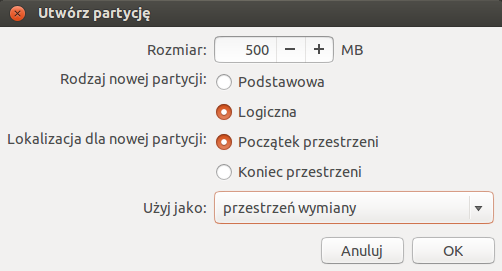
\includegraphics[width=\linewidth]{images/instalator_partycjonowanie_gparted_dodaj_swap.png}
	\caption*{Ustawienia dla partycji wymiany (swap).}
\end{wrapfigure}

Teraz utwórz partycję wymiany. Więcej o tej partycji przeczytasz w w sekcji \ref{ile_miejsca} ,,Ile miejsca przeznaczyć na Ubuntu''. Pozostałe opcje ustaw jak na rysunku. Kliknij przycisk \textcolor{ubuntu_orange}{OK}, aby utworzyć nową partycję.

\begin{wrapfigure}{R}{0.5\textwidth}
	\vspace{-10pt}
	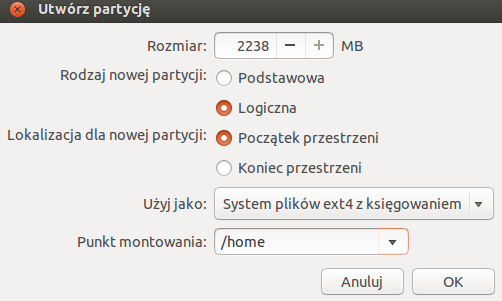
\includegraphics[width=\linewidth]{images/instalator_partycjonowanie_gparted_dodaj_home.png}
	\caption*{Ustawienia dla partycji domowej (/home).}
\end{wrapfigure}

Na koniec pozostało utworzenie partycji domowej. Więcej o tej partycji przeczytasz w sekcji \ref{ile_miejsca} ,,Ile miejsca przeznaczyć na Ubuntu''. Pozostałe opcje ustaw jak na rysunku. Kliknij przycisk \textcolor{ubuntu_orange}{OK}, aby utworzyć nową partycję.

\begin{center}
	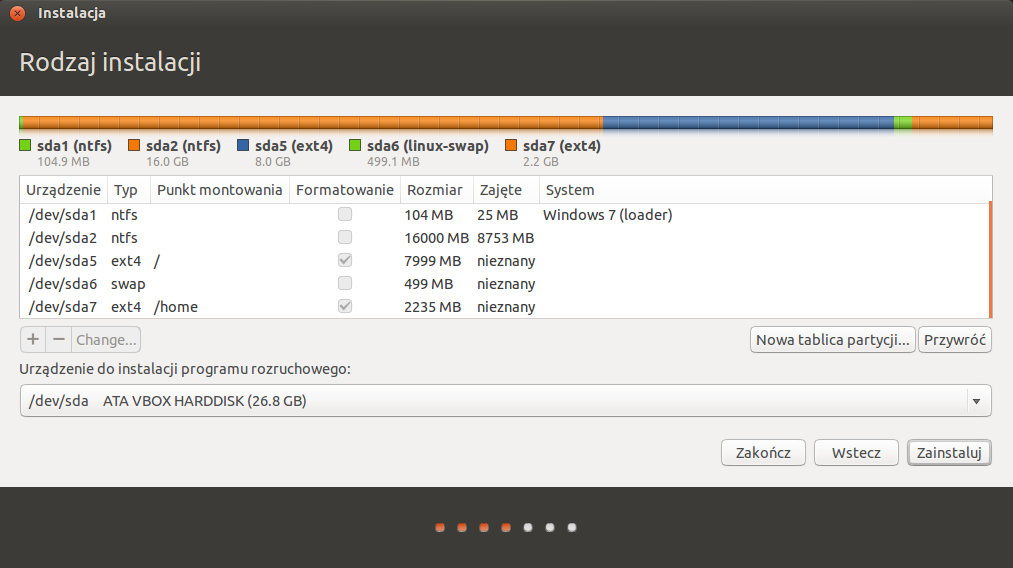
\includegraphics[width=\linewidth]{images/instalator_partycjonowanie_gparted4.png}
\end{center}

Ekran programu GParted wygląda teraz mniej więcej tak, jak na rysunku powyżej. Masz dwie partycje systemu Windows (NTFS), partycję wymiany systemu Linux (swap) oraz dwie partycje dla systemu Ubuntu (ext4). Upewnij się, że partycje NTFS \textcolor{ubuntu_orange}{nie} są zaznaczone do sformatowania, zaś partycje ext4 tak.

Kliknij przycisk \textcolor{ubuntu_orange}{Naprzód}, aby wprowadzić zmiany na partycjach.\\
Teraz możesz powrócić do lektury procesu instalacji w miejscu, gdzie go przerwałeś.\\
Powrót do \ref{instalator_strefa_czasowa}: ,,Wybór strefy czasowej''.
\clearpage
